\documentclass[12pt]{article}
\usepackage[left=2cm, top=2cm, right=2cm, bottom=2cm]{geometry}
\usepackage[utf8]{inputenc}      % accents dans le source
\usepackage[T1]{fontenc}
\usepackage[french]{babel}
\usepackage{graphicx}
\usepackage{graphics}
\usepackage{amsmath}
\usepackage{amsfonts}
\usepackage{amssymb}
\usepackage{tikz}
\usepackage{xcolor} 
\usepackage{mathtools}
\usepackage{parskip}
\usepackage{subcaption}
\usepackage[export]{adjustbox}
\usepackage{hyperref}

\tikzset{every picture/.style={line width=0.75pt}}
\newcommand{\sinc}{\operatorname{sinc}}


\title{\textbf{Optique ondulatoire:} Diffraction de la lumière}
\author{MENARD Alexandre - VIEILLEDENT Florent}

\setlength{\parindent}{1cm}

\begin{document}
\maketitle

\section*{Introduction}

\break
\section{Diffraction par des ouvertures simples}
Dans cette première partie, nous nous intéressons au cas de la diffraction dans le cas d'ouvertures simples. Nous y proposerons une description qualitative, quantitative dans le cas d'une fente simple,
une description de motifs de diffraction pour différentes ouvertures. Enfin, nous proposerons un protocole permettant de déterminer avec précision le diamètre d'un cheveu en s'appuyant sur le théorème de Babinet.
\subsection{Etude d'une fente simple de largeur variable}
Pour une première approche, nous installons un laser face à un écran, et l'on insère une fente simple de largeur variable $a$ entre le laser et l'écran, à un distance $D$ de l'écran.
\begin{figure}[!h]
    \begin{center}
        \resizebox{0.7\textwidth}{5cm}{
        \begin{tikzpicture}[x=0.75pt,y=0.75pt,yscale=-1,xscale=1]
%uncomment if require: \path (0,300); %set diagram left start at 0, and has height of 300

%Flowchart: Process [id:dp872954957901976] 
\draw   (104,140) -- (184,140) -- (184,160) -- (104,160) -- cycle ;
%Straight Lines [id:da9241077852973352] 
\draw [color={rgb, 255:red, 208; green, 2; blue, 27 }  ,draw opacity=1 ][line width=0.75]    (184,150) -- (354,150) ;
\draw [shift={(275,150)}, rotate = 180] [color={rgb, 255:red, 208; green, 2; blue, 27 }  ,draw opacity=1 ][line width=0.75]    (10.93,-3.29) .. controls (6.95,-1.4) and (3.31,-0.3) .. (0,0) .. controls (3.31,0.3) and (6.95,1.4) .. (10.93,3.29)   ;
%Straight Lines [id:da39324764499965714] 
\draw    (354,160) -- (354,200) ;
%Straight Lines [id:da3239950960426152] 
\draw    (354,100) -- (354,140) ;
%Straight Lines [id:da8041456916959207] 
\draw [color={rgb, 255:red, 208; green, 2; blue, 27 }  ,draw opacity=1 ]   (354,150) -- (534,130) ;
\draw [shift={(449.96,139.34)}, rotate = 173.66] [color={rgb, 255:red, 208; green, 2; blue, 27 }  ,draw opacity=1 ][line width=0.75]    (10.93,-3.29) .. controls (6.95,-1.4) and (3.31,-0.3) .. (0,0) .. controls (3.31,0.3) and (6.95,1.4) .. (10.93,3.29)   ;
%Straight Lines [id:da7837201764569335] 
\draw [color={rgb, 255:red, 208; green, 2; blue, 27 }  ,draw opacity=1 ]   (354,150) -- (534,170) ;
\draw [shift={(449.96,160.66)}, rotate = 186.34] [color={rgb, 255:red, 208; green, 2; blue, 27 }  ,draw opacity=1 ][line width=0.75]    (10.93,-3.29) .. controls (6.95,-1.4) and (3.31,-0.3) .. (0,0) .. controls (3.31,0.3) and (6.95,1.4) .. (10.93,3.29)   ;
%Straight Lines [id:da08364499364029099] 
\draw  [dash pattern={on 0.84pt off 2.51pt}]  (354,150) -- (534,150) ;
%Straight Lines [id:da3720582141386004] 
\draw    (534,100) -- (534,200) ;
%Straight Lines [id:da4573530253324263] 
\draw    (366,240) -- (522,240) ;
\draw [shift={(524,240)}, rotate = 180] [color={rgb, 255:red, 0; green, 0; blue, 0 }  ][line width=0.75]    (10.93,-3.29) .. controls (6.95,-1.4) and (3.31,-0.3) .. (0,0) .. controls (3.31,0.3) and (6.95,1.4) .. (10.93,3.29)   ;
\draw [shift={(364,240)}, rotate = 0] [color={rgb, 255:red, 0; green, 0; blue, 0 }  ][line width=0.75]    (10.93,-3.29) .. controls (6.95,-1.4) and (3.31,-0.3) .. (0,0) .. controls (3.31,0.3) and (6.95,1.4) .. (10.93,3.29)   ;
%Straight Lines [id:da5804934197531184] 
\draw    (554,132) -- (554,168) ;
\draw [shift={(554,170)}, rotate = 270] [color={rgb, 255:red, 0; green, 0; blue, 0 }  ][line width=0.75]    (10.93,-3.29) .. controls (6.95,-1.4) and (3.31,-0.3) .. (0,0) .. controls (3.31,0.3) and (6.95,1.4) .. (10.93,3.29)   ;
\draw [shift={(554,130)}, rotate = 90] [color={rgb, 255:red, 0; green, 0; blue, 0 }  ][line width=0.75]    (10.93,-3.29) .. controls (6.95,-1.4) and (3.31,-0.3) .. (0,0) .. controls (3.31,0.3) and (6.95,1.4) .. (10.93,3.29)   ;

% Text Node
\draw (125,142) node [anchor=north west][inner sep=0.75pt]   [align=left] {Laser};
% Text Node
\draw (305,49) node [anchor=north west][inner sep=0.75pt]   [align=left] {Fente simple\\de largeur $\displaystyle a$};
% Text Node
\draw (438,212.4) node [anchor=north west][inner sep=0.75pt]    {$D$};
% Text Node
\draw (565,142.4) node [anchor=north west][inner sep=0.75pt]    {$L$};
% Text Node
\draw (515,62) node [anchor=north west][inner sep=0.75pt]   [align=left] {Ecran};


\end{tikzpicture}

        }
    \end{center}
    \caption{Schéma du montage}
    \label{fig:montage_simple}
\end{figure}

Pour une largeur fixe, nous observons une figure de diffraction avec une large tâche centrale, puis des zéros d'intensité et de nouvelles tâches qui se répetent de chaque côté de la tâche centrale.
En augmentant la largeur de la fente $a$, nous observons un resserement des tâches d'intensité maximale et lorsque l'on réduit la largeur, ces mêmes tâches s'élargissent.\footnote{Les photos sont prises à même distance sans changement de focale, les échelles sont donc identiques d'une photo à l'autre}

\begin{figure}[h!]
    \centering
    \begin{subfigure}{.33\textwidth}
      \centering
        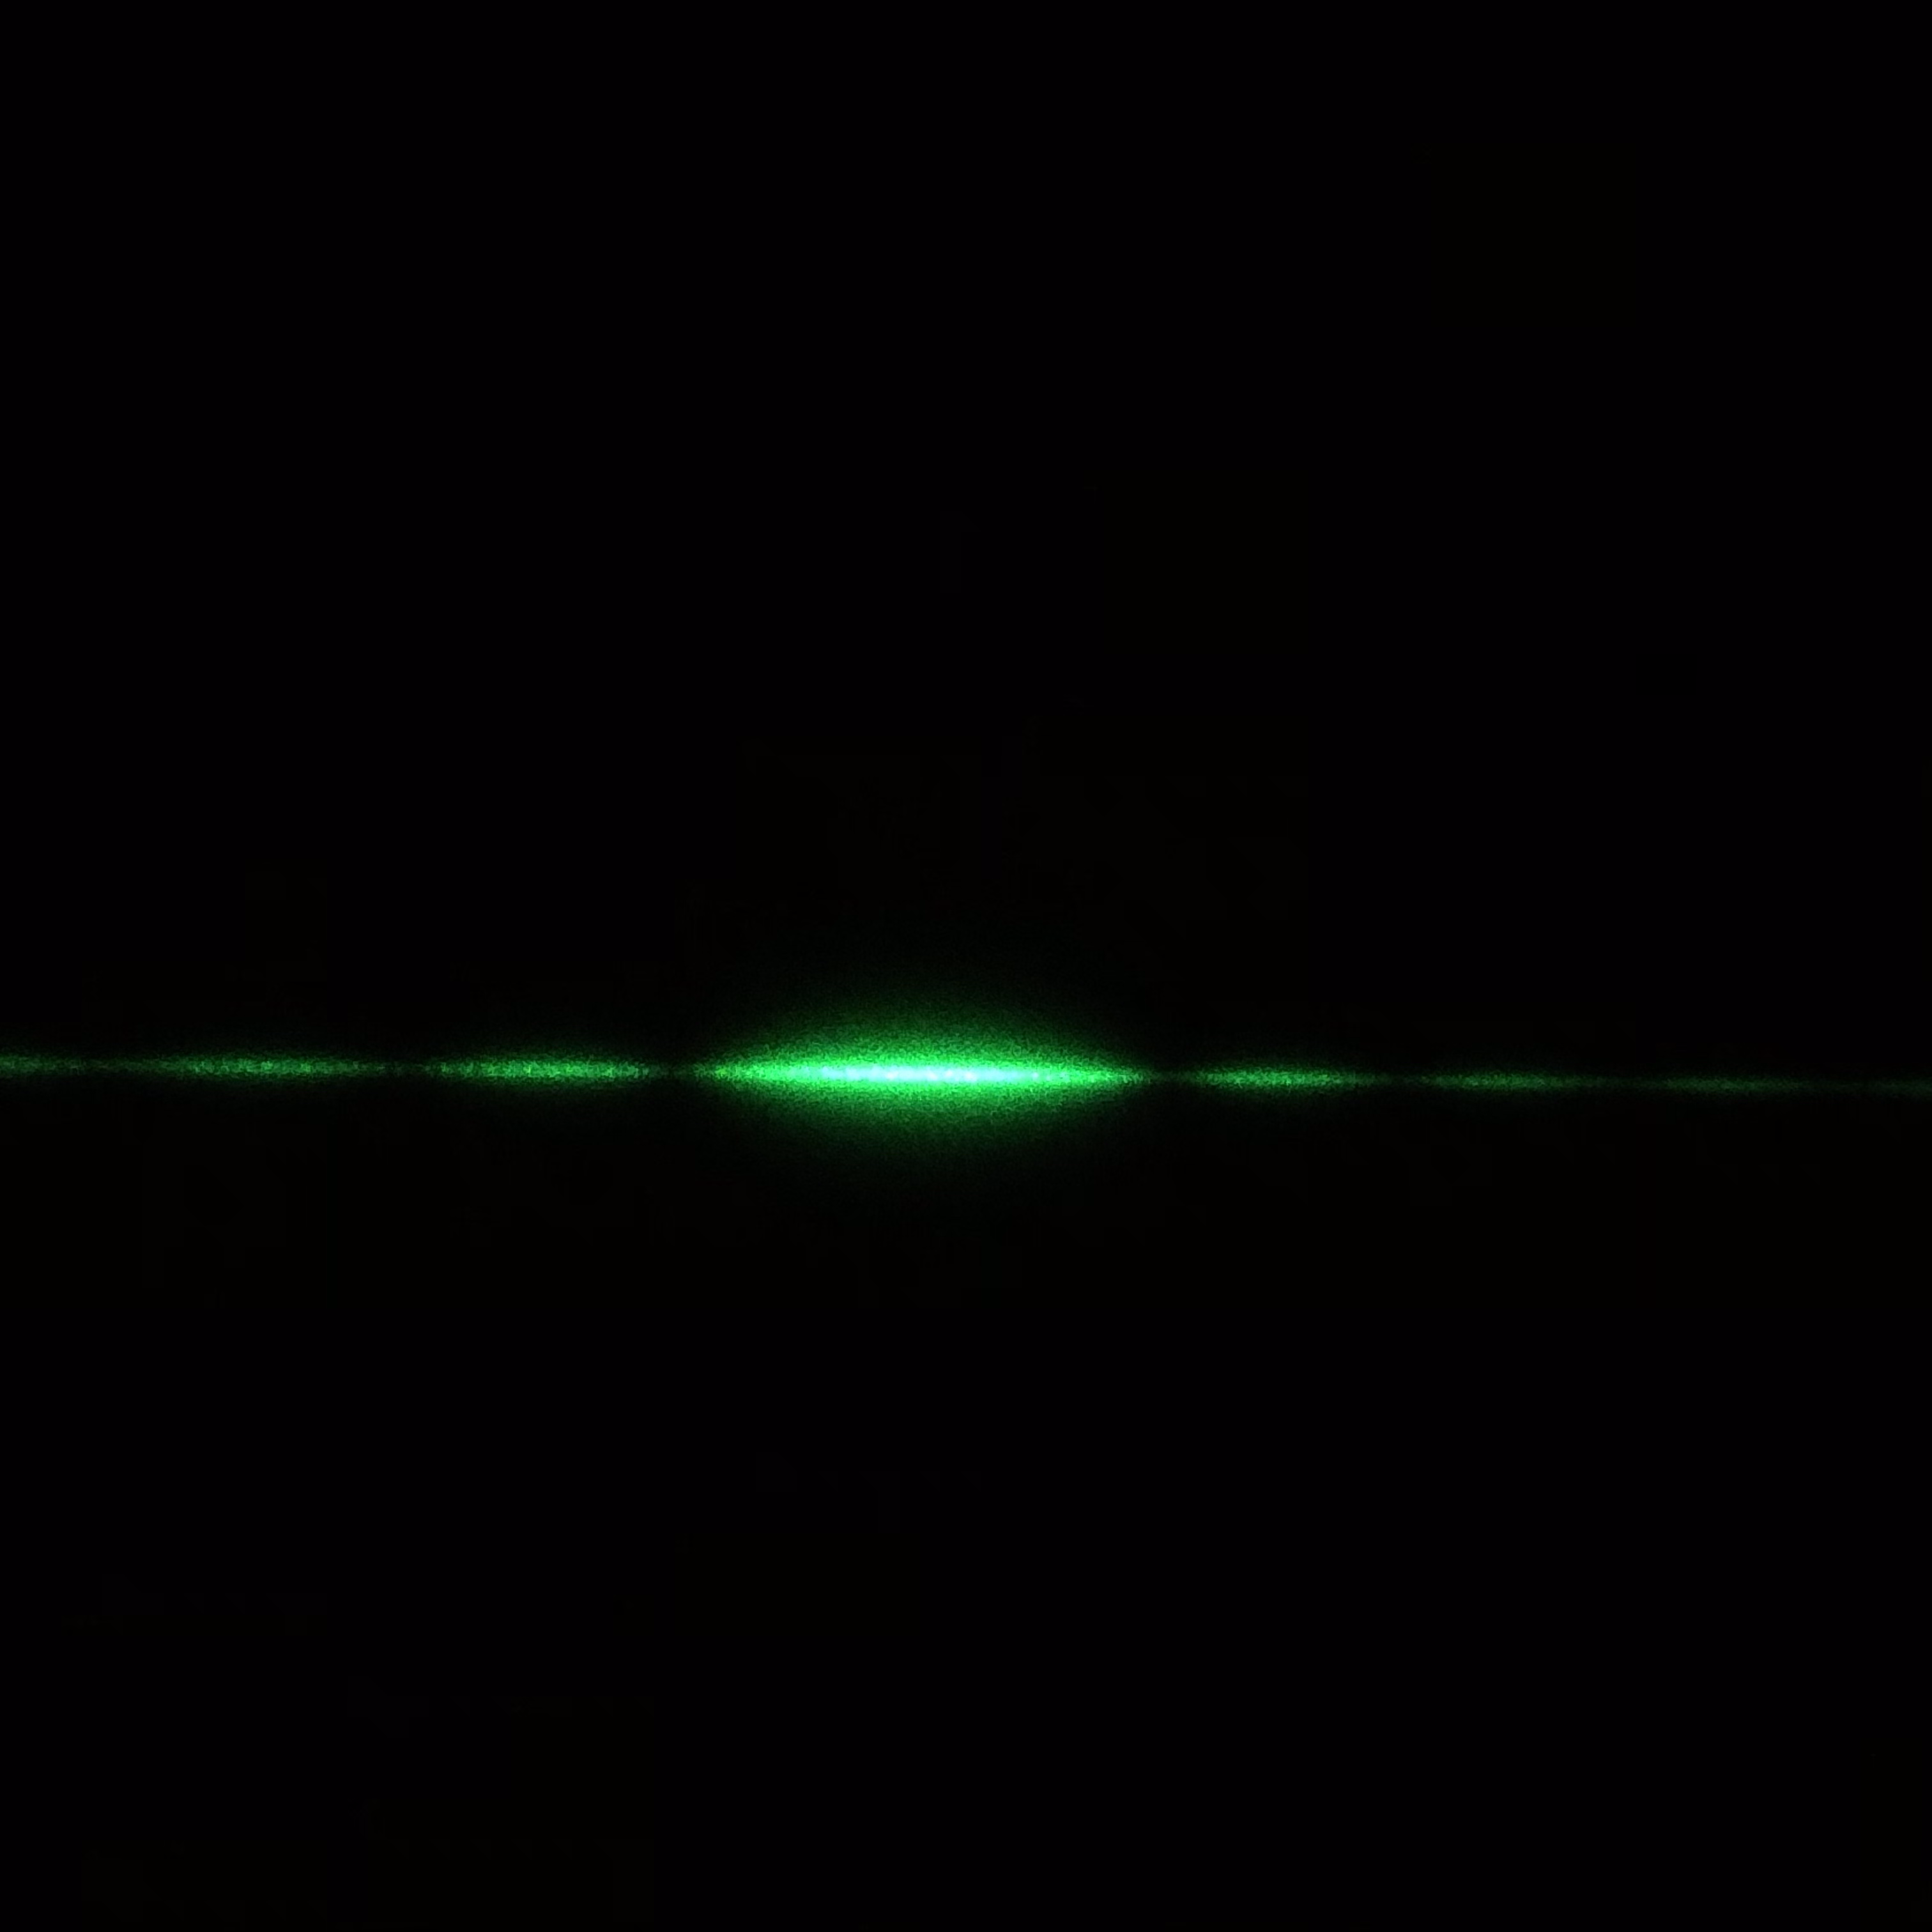
\includegraphics[width=.9\linewidth]{img/diffrac_simple_a_diminu.png}
      \caption{Largeur $a$ qui diminue}
      \label{fig:sfig1}
    \end{subfigure}%
    \begin{subfigure}{.33\textwidth}
      \centering
      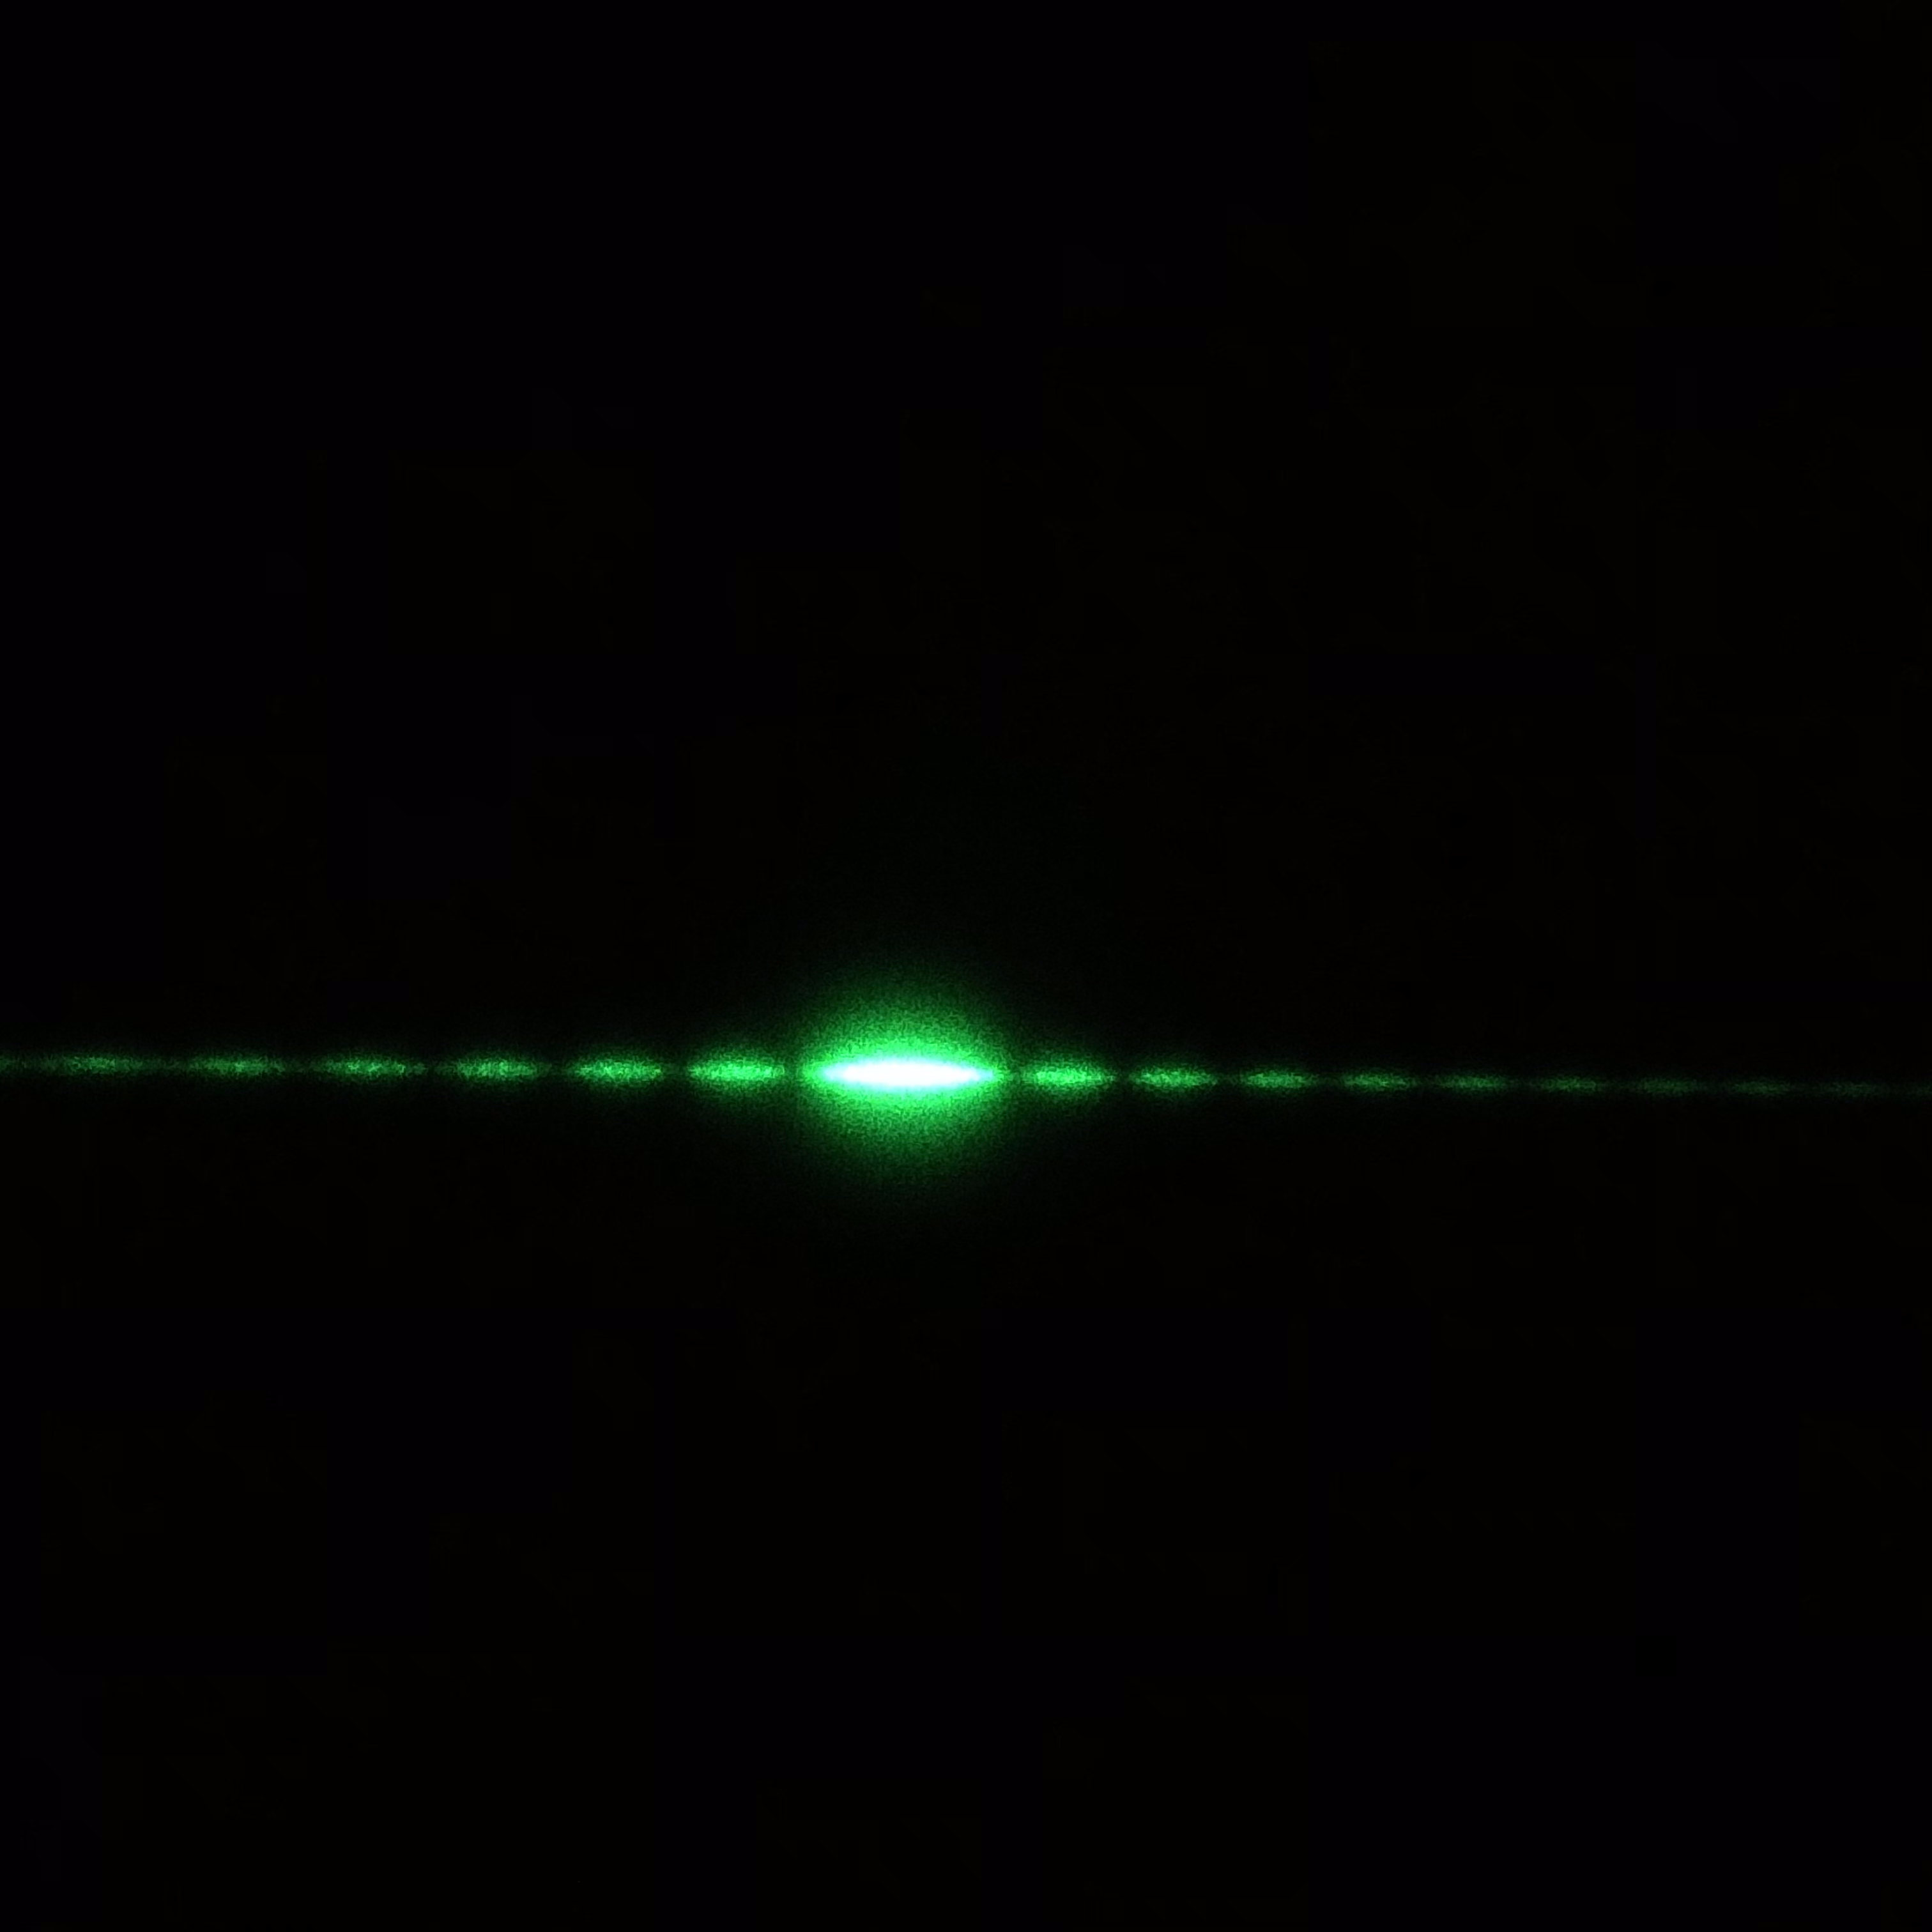
\includegraphics[width=.9\linewidth]{img/driffac_simple_centre.png}
      \caption{Largeur $a$ initiale}
      \label{fig:sfig2}
    \end{subfigure}
    \begin{subfigure}{.33\textwidth}
        \centering
        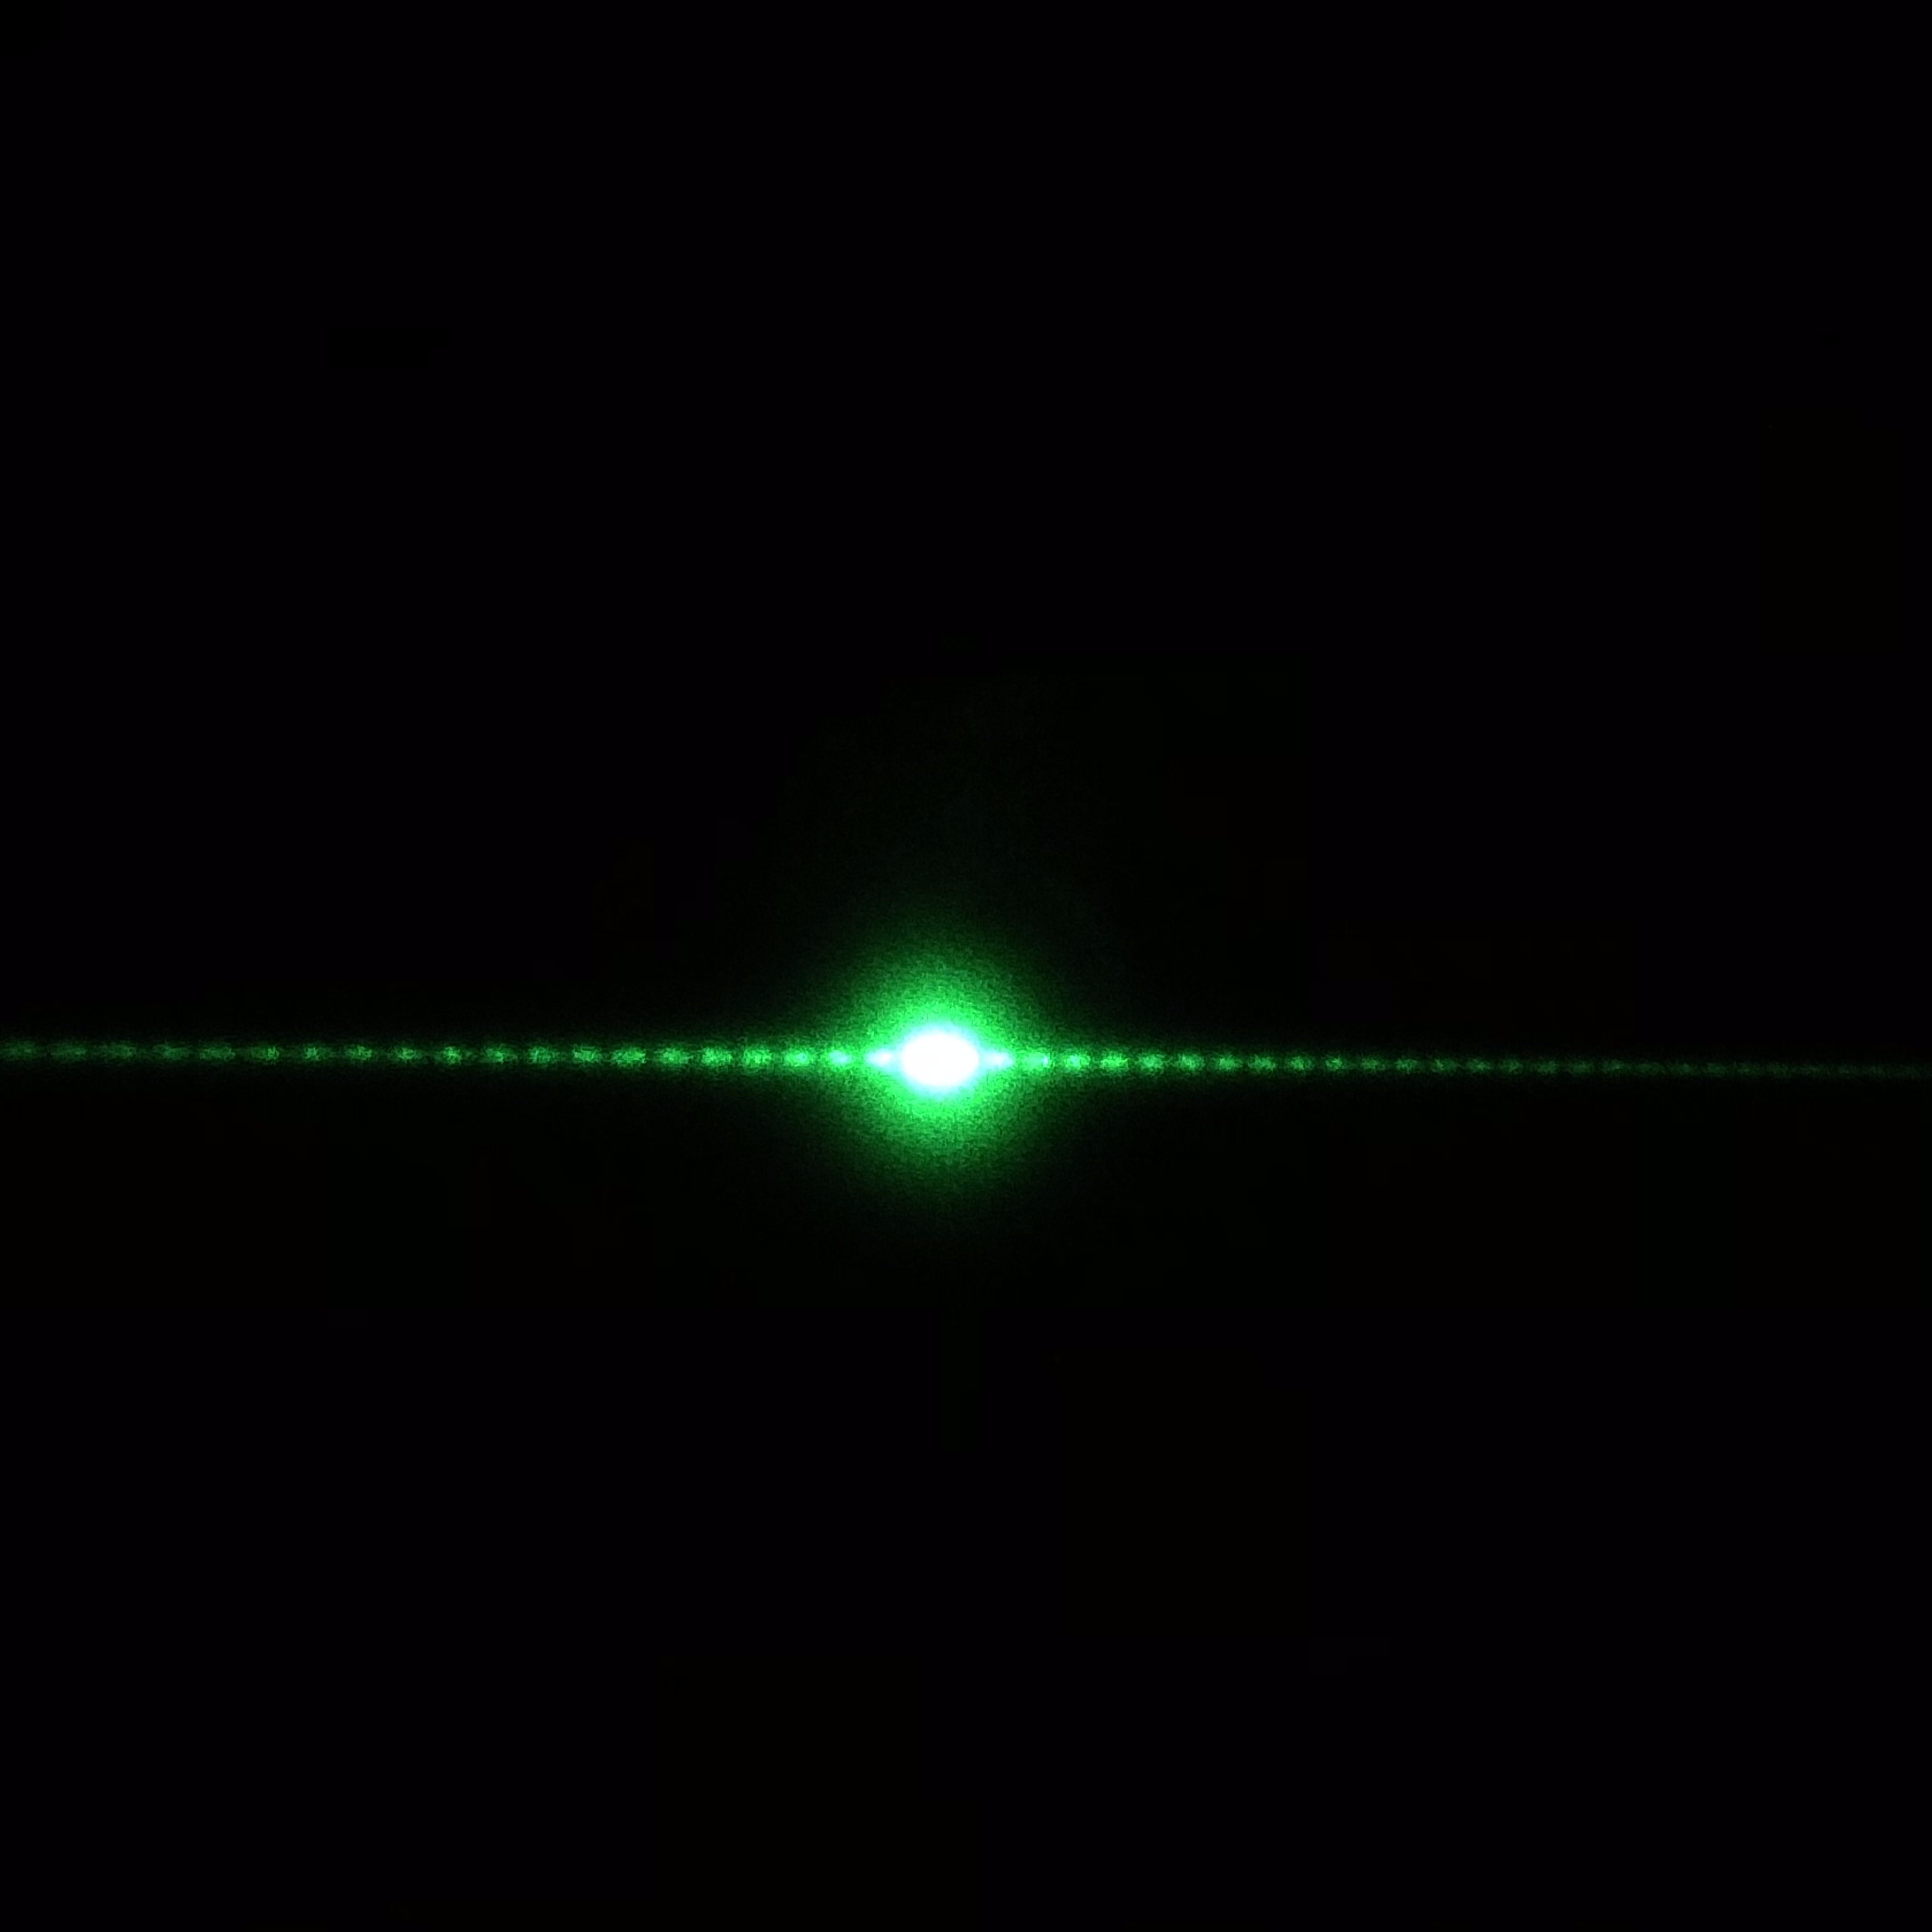
\includegraphics[width=.9\linewidth]{img/diffrac_simple_a_augmente.png}
        \caption{Largeur $a$ qui augmente}
        \label{fig:sfig3}
      \end{subfigure}
    \caption{Figure de diffraction en fonction de la largeur de la fente}
    \label{fig:fig}
\end{figure}

\break
Nous proposons ensuite de vérifier la formule qui donne la largeur de la tâche centrale $L$ pour des configurations différentes de $\lambda, D$ et $a$. Pour cela, nous devons
connaître les valeurs d'annulation de l'intensité en fonction de $y$.
\begin{align*}
    I(\theta) = I_0 \sinc^2\left(\frac{\pi a \sin \theta}{\lambda}\right) = 0 & \Leftrightarrow \sinc\left(\frac{\pi a \sin \theta}{\lambda}\right) = 0 \\
    & \Leftrightarrow \frac{\pi a \sin \theta}{\lambda} = n\pi, \forall n \in \mathbb{Z}^* \\
    & \Leftrightarrow \sin \theta = \frac{n\lambda}{a}
\end{align*}

Dans le cadre où $\theta$ très petit, on a $\theta \approx \sin \theta \approx \tan \theta $ et $\tan \theta = \frac{y}{D}$, il vient que:
\begin{align}
    \label{eqn:loi_intensite}
    y_n = \frac{n\lambda D}{a}, \forall n \in \mathbb{Z}^*
\end{align}

On peut alors en déduire la largeur $L$ de la tâche centrale qui s'étend entre les deux premiers minimums $n=1$ et $n=-1$ d'où:
\begin{align}
    \label{eqn:loi_L}
    L = \left\lvert y_{-1} - y_1 \right\rvert = \frac{2\lambda D}{a}
\end{align}

Pour vérifier cette loi (\ref{eqn:loi_intensite}), nous allons utiliser un seul et même montage, mais nous ferons varier un paramètre à la fois à savoir la longueur d'onde $\lambda$, la distance entre la fente et l'écran $D$, 
et la largeur de la fente $a$ montée sur un support d'épaisseur $e = 1.2 \pm 0.1cm$. Pour cela, nous plaçons un laser de longueur d'onde $\lambda$ face à un écran, et une fente de largeur $a$ entre les deux à une distance $D$ de l'écran.

\begin{figure}[!h]
    \begin{center}
        \resizebox{0.7\textwidth}{5cm}{
        
\begin{tikzpicture}[x=0.75pt,y=0.75pt,yscale=-1,xscale=1]
%uncomment if require: \path (0,300); %set diagram left start at 0, and has height of 300

%Flowchart: Process [id:dp6086218837893427] 
\draw   (60,140) -- (140,140) -- (140,160) -- (60,160) -- cycle ;
%Straight Lines [id:da38385449858597576] 
\draw [color={rgb, 255:red, 208; green, 2; blue, 27 }  ,draw opacity=1 ][line width=0.75]    (140,150) -- (310,150) ;
\draw [shift={(231,150)}, rotate = 180] [color={rgb, 255:red, 208; green, 2; blue, 27 }  ,draw opacity=1 ][line width=0.75]    (10.93,-3.29) .. controls (6.95,-1.4) and (3.31,-0.3) .. (0,0) .. controls (3.31,0.3) and (6.95,1.4) .. (10.93,3.29)   ;
%Straight Lines [id:da8505256469428157] 
\draw [color={rgb, 255:red, 208; green, 2; blue, 27 }  ,draw opacity=1 ]   (310,150) -- (490,130) ;
\draw [shift={(405.96,139.34)}, rotate = 173.66] [color={rgb, 255:red, 208; green, 2; blue, 27 }  ,draw opacity=1 ][line width=0.75]    (10.93,-3.29) .. controls (6.95,-1.4) and (3.31,-0.3) .. (0,0) .. controls (3.31,0.3) and (6.95,1.4) .. (10.93,3.29)   ;
%Straight Lines [id:da09375676890060713] 
\draw [color={rgb, 255:red, 208; green, 2; blue, 27 }  ,draw opacity=1 ]   (310,150) -- (490,170) ;
\draw [shift={(405.96,160.66)}, rotate = 186.34] [color={rgb, 255:red, 208; green, 2; blue, 27 }  ,draw opacity=1 ][line width=0.75]    (10.93,-3.29) .. controls (6.95,-1.4) and (3.31,-0.3) .. (0,0) .. controls (3.31,0.3) and (6.95,1.4) .. (10.93,3.29)   ;
%Straight Lines [id:da6004144363266697] 
\draw  [dash pattern={on 0.84pt off 2.51pt}]  (310,150) -- (490,150) ;
%Straight Lines [id:da19124540000034584] 
\draw    (490,100) -- (490,200) ;
%Straight Lines [id:da2398039016356004] 
\draw  [dash pattern={on 0.84pt off 2.51pt}]  (310,200) -- (310,230) ;
%Shape: Rectangle [id:dp37982021323713533] 
\draw   (300,100) -- (320,100) -- (320,140) -- (300,140) -- cycle ;
%Shape: Rectangle [id:dp9665691920024131] 
\draw   (300,160) -- (320,160) -- (320,200) -- (300,200) -- cycle ;
%Straight Lines [id:da33860911421706397] 
\draw    (310,140) -- (310,160) ;
%Straight Lines [id:da9593511627291105] 
\draw    (260,210) -- (298,210) ;
\draw [shift={(300,210)}, rotate = 180] [color={rgb, 255:red, 0; green, 0; blue, 0 }  ][line width=0.75]    (10.93,-3.29) .. controls (6.95,-1.4) and (3.31,-0.3) .. (0,0) .. controls (3.31,0.3) and (6.95,1.4) .. (10.93,3.29)   ;
%Straight Lines [id:da6509863973529162] 
\draw    (280,230) -- (520,230) (283,226) -- (283,234)(286,226) -- (286,234)(289,226) -- (289,234)(292,226) -- (292,234)(295,226) -- (295,234)(298,226) -- (298,234)(301,226) -- (301,234)(304,226) -- (304,234)(307,226) -- (307,234)(310,226) -- (310,234)(313,226) -- (313,234)(316,226) -- (316,234)(319,226) -- (319,234)(322,226) -- (322,234)(325,226) -- (325,234)(328,226) -- (328,234)(331,226) -- (331,234)(334,226) -- (334,234)(337,226) -- (337,234)(340,226) -- (340,234)(343,226) -- (343,234)(346,226) -- (346,234)(349,226) -- (349,234)(352,226) -- (352,234)(355,226) -- (355,234)(358,226) -- (358,234)(361,226) -- (361,234)(364,226) -- (364,234)(367,226) -- (367,234)(370,226) -- (370,234)(373,226) -- (373,234)(376,226) -- (376,234)(379,226) -- (379,234)(382,226) -- (382,234)(385,226) -- (385,234)(388,226) -- (388,234)(391,226) -- (391,234)(394,226) -- (394,234)(397,226) -- (397,234)(400,226) -- (400,234)(403,226) -- (403,234)(406,226) -- (406,234)(409,226) -- (409,234)(412,226) -- (412,234)(415,226) -- (415,234)(418,226) -- (418,234)(421,226) -- (421,234)(424,226) -- (424,234)(427,226) -- (427,234)(430,226) -- (430,234)(433,226) -- (433,234)(436,226) -- (436,234)(439,226) -- (439,234)(442,226) -- (442,234)(445,226) -- (445,234)(448,226) -- (448,234)(451,226) -- (451,234)(454,226) -- (454,234)(457,226) -- (457,234)(460,226) -- (460,234)(463,226) -- (463,234)(466,226) -- (466,234)(469,226) -- (469,234)(472,226) -- (472,234)(475,226) -- (475,234)(478,226) -- (478,234)(481,226) -- (481,234)(484,226) -- (484,234)(487,226) -- (487,234)(490,226) -- (490,234)(493,226) -- (493,234)(496,226) -- (496,234)(499,226) -- (499,234)(502,226) -- (502,234)(505,226) -- (505,234)(508,226) -- (508,234)(511,226) -- (511,234)(514,226) -- (514,234)(517,226) -- (517,234) ;
%Straight Lines [id:da49975530995593975] 
\draw  [dash pattern={on 0.84pt off 2.51pt}]  (490,200) -- (490,230) ;
%Straight Lines [id:da26109354701785903] 
\draw    (550,210) -- (502,210) ;
\draw [shift={(500,210)}, rotate = 360] [color={rgb, 255:red, 0; green, 0; blue, 0 }  ][line width=0.75]    (10.93,-3.29) .. controls (6.95,-1.4) and (3.31,-0.3) .. (0,0) .. controls (3.31,0.3) and (6.95,1.4) .. (10.93,3.29)   ;
%Straight Lines [id:da7931027821198187] 
\draw    (300,90) -- (320,90) ;
\draw [shift={(320,90)}, rotate = 180] [color={rgb, 255:red, 0; green, 0; blue, 0 }  ][line width=0.75]    (0,5.59) -- (0,-5.59)   ;
\draw [shift={(300,90)}, rotate = 180] [color={rgb, 255:red, 0; green, 0; blue, 0 }  ][line width=0.75]    (0,5.59) -- (0,-5.59)   ;
%Straight Lines [id:da5127007685927278] 
\draw    (322,220) -- (478,220) ;
\draw [shift={(480,220)}, rotate = 180] [color={rgb, 255:red, 0; green, 0; blue, 0 }  ][line width=0.75]    (10.93,-3.29) .. controls (6.95,-1.4) and (3.31,-0.3) .. (0,0) .. controls (3.31,0.3) and (6.95,1.4) .. (10.93,3.29)   ;
\draw [shift={(320,220)}, rotate = 0] [color={rgb, 255:red, 0; green, 0; blue, 0 }  ][line width=0.75]    (10.93,-3.29) .. controls (6.95,-1.4) and (3.31,-0.3) .. (0,0) .. controls (3.31,0.3) and (6.95,1.4) .. (10.93,3.29)   ;
%Straight Lines [id:da9902733058999353] 
\draw    (500,132) -- (500,168) ;
\draw [shift={(500,170)}, rotate = 270] [color={rgb, 255:red, 0; green, 0; blue, 0 }  ][line width=0.75]    (10.93,-3.29) .. controls (6.95,-1.4) and (3.31,-0.3) .. (0,0) .. controls (3.31,0.3) and (6.95,1.4) .. (10.93,3.29)   ;
\draw [shift={(500,130)}, rotate = 90] [color={rgb, 255:red, 0; green, 0; blue, 0 }  ][line width=0.75]    (10.93,-3.29) .. controls (6.95,-1.4) and (3.31,-0.3) .. (0,0) .. controls (3.31,0.3) and (6.95,1.4) .. (10.93,3.29)   ;

% Text Node
\draw (74,140) node [anchor=north west][inner sep=0.75pt]   [align=left] {Laser $\displaystyle \lambda $};
% Text Node
\draw (252,22) node [anchor=north west][inner sep=0.75pt]   [align=left] {Support de fente\\avec jeton A3015};
% Text Node
\draw (471,62) node [anchor=north west][inner sep=0.75pt]   [align=left] {Ecran};
% Text Node
\draw (191,192) node [anchor=north west][inner sep=0.75pt]   [align=left] {\begin{minipage}[lt]{40.7pt}\setlength\topsep{0pt}
\begin{center}
Règle\\verticale
\end{center}

\end{minipage}};
% Text Node
\draw (551,192) node [anchor=north west][inner sep=0.75pt]   [align=left] {\begin{minipage}[lt]{40.7pt}\setlength\topsep{0pt}
\begin{center}
Règle\\verticale
\end{center}

\end{minipage}};
% Text Node
\draw (296,251) node [anchor=north west][inner sep=0.75pt]   [align=left] {Règle à plat sur le banc optique};
% Text Node
\draw (306,68.4) node [anchor=north west][inner sep=0.75pt]    {$e$};
% Text Node
\draw (391,192.4) node [anchor=north west][inner sep=0.75pt]    {$D$};
% Text Node
\draw (511,142.4) node [anchor=north west][inner sep=0.75pt]    {$L$};


\end{tikzpicture}

        }
    \end{center}
    \caption{Schéma du montage}
\end{figure}

Pour relever la distance $D$ entre l'écran et la fente, nous disposons une règle précise au 1/2 mm à plat sur le banc optique, et nous relevons la position $x_1$ de la fente en plaçant une petite règle verticale au centre de l'épaisseur $e$ du support, et l'on 
relève la mesure sur la règle à plat. Pour la position $x_2$ de l'écran, nous suivons le même procédé en collant à plat la règle contre l'écran. 
L'incertitude sur la position de la fente est donc de $\delta x_1 = e/2 = 0.6cm$ car l'on ne sait pas si la fente est parfaitement centrée dans le support, et pour l'écran on a $\delta x_2 = 0.2cm$. Ainsi, on obtient $D$ avec:
\begin{align}
    D = \left\lvert x_2 - x_1\right\rvert, \quad \delta D = \delta x_1 + \delta x_2 = 0.8cm
\end{align}

L'incertitude sur la longueur d'onde est typiquement de l'ordre de $\delta \lambda = 10nm$ pour des lasers de cette gamme de longueur d'onde. Les fentes sont précises au $\mu m$ d'après le constructeur,
nous avons donc $\delta a = 1 \mu m$. Enfin pour le relevé de la largeur de la tâche centrale, nous utilisons une règle précise au 1/2 mm, et nous mesurons la distance entre les centres des deux tâches noires
de part et d'autre de la tâche centrale, l'incertitude sur une position d'une tâche noire vaut la moitié de sa largeur, et comme l'on effectue une différence pour obtenir $L$, les incertitudes s'additionnent. L'incertitude sur $L$ est donc 
la largeur d'une des tâches noires.

\subsubsection{Influence de la largeur de la fente}
Pour ce premier paramètre, nous allons placer différentes fentes de largeur $a$ calibrée à une distance $D = 75.5 \pm 0.8 cm$ de l'écran, et l'on illumine les différentes fentes avec un laser de longueur d'onde
$\lambda = 532 \pm 10nm$ (laser vert). 

\begin{table}[h!]
	\centering
	\begin{tabular}{||c c||} 
		\hline
		$a \pm 0.1 \mu m$ & $L_{exp}$ en cm \\
		\hline\hline
		\footnotesize
        $200$   &  $0.40     \pm 0.05$ \\ 
        $150$   &  $0.55    \pm 0.05$ \\ 
        $100$   &  $0.75    \pm 0.05$ \\ 
        $80$    &  $1.05    \pm 0.05$ \\ 
        $60$    &  $1.35    \pm 0.05$ \\ 
        $40$    &  $2.1     \pm 0.1$ \\ 
        $30$    &  Mesure impossible \\ 
		\hline
	\end{tabular}
	\caption{Mesure de $L_{exp}$ pour une largeur de fente variable}
	\label{table:1}
\end{table}

La mesure à $a = 30\mu m$ était impossible car l'on ne réussissait pas à faire passer le laser sur la fente en question trop à gauche sur le jeton, donc le faisceau du laser heurtait le support. 

Pour une première analyse, nous pouvons remarquer que si $a$ diminue, la tâche centrale $L$ augmente, ce qui est en accord avec la théorie.

\subsubsection{Influence de la longueur d'onde}
Pour ce second paramètre, nous fixons une fente de largeur $a = 80 \pm 1 \mu m$ calibrée, à une distance $D = 75.5 \pm 0.8 cm$ de l'écran, et l'on placera différents laser de longueur d'onde $\lambda = 650, 532, 450 \pm 10nm$ (rouge, vert, bleu).

\begin{table}[h!]
	\centering
	\begin{tabular}{||c c||} 
		\hline
		$\lambda \pm 10 nm$ & $L_{exp}$ en cm \\
		\hline\hline
		\footnotesize
        $650$   &  $1.20 \pm 0.05$ \\ 
        $532$   &  $1.00 \pm 0.05$ \\ 
        $450$   &  $0.75 \pm 0.05$ \\ 
		\hline
	\end{tabular}
	\caption{Mesure de $L_{exp}$ pour une longueur d'onde variable}
	\label{table:2}
\end{table}

Nous remarquons que la largeur de la tâche suit le comportement prédit par la théorie à savoir que plus $\lambda$ est grand, plus la taille de la tâche centrale est grande.

\break
\subsubsection{Influence de la distance entre l'écran et la fente}
Pour ce dernier paramètre, nous illuminons une fente de largeur $a = 40 \pm 1 \mu m$ calibrée, avec un laser de longueur d'onde $\lambda = 532 \pm 10 nm$ et nous allons faire varier la distance $D$ entre la fente et l'écran.

\begin{table}[h!]
	\centering
	\begin{tabular}{||c c||} 
		\hline
		$D \pm 0.5 cm$ & $L_{exp}$ en cm \\
		\hline\hline
		\footnotesize
        $75.5$      &  $2.0 \pm 0.1$ \\ 
        $65.5$      &  $1.75 \pm 0.05$ \\ 
        $55$        &  $1.45 \pm 0.05$ \\ 
        $45.5$      &  $1.25 \pm 0.05$ \\ 
        $35.2$      &  $0.95 \pm 0.05$ \\ 
        $25$        &  $0.6 \pm 0.05$ \\ 
        $15$        &  $0.35 \pm 0.05$ \\ 
        $5$         &  Mesure impossible \\ 
		\hline
	\end{tabular}
	\caption{Mesure de $L_{exp}$ pour une distance fente-écran variable}
	\label{table:3}
\end{table}

La mesure à $D = 5cm$ était trop complexe à obtenir de par la très faible taille de la largeur centrale, la mesure n'aurait donc pas plus être précise et serait inutilisable pour l'analyse des résultats.

Ici, quand $D$ augmente, la largeur de la tâche centrale augmente, ce qui est aussi prédit par la théorie. Il nous faut cependant vérifier la justesse de la théorie quantitativement.

\subsubsection{Synthèse et analyse des résultats expérimentaux}
Nous réunissons l'ensemble de nos mesures dans un graphique de la largeur expérimentale $L_{exp}$ en fonction de la largeur théorique $L_{th}$, de telle sorte à disposer l'ensemble des points 
sur une droite d'équation $y=x$ pour mettre en évidence des écarts entre l'expérience et la théorie. 

\begin{figure}[!h]
    \begin{center}
        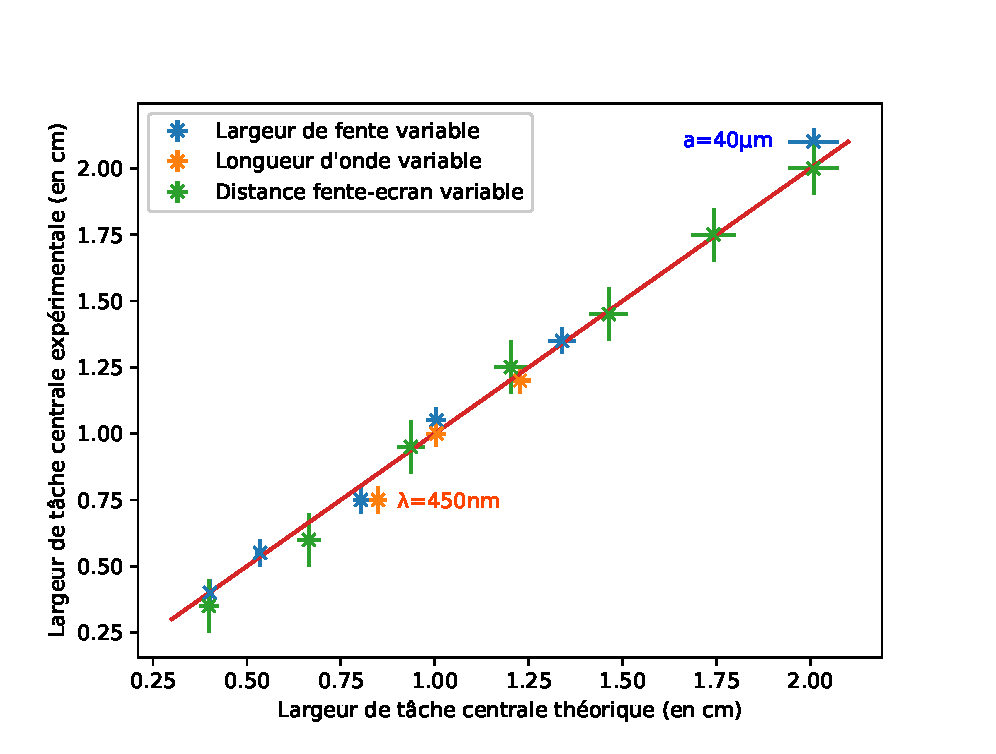
\includegraphics[scale=0.65]{img/graph_final_diffrac_simple.eps}
    \end{center}
    \caption{Graphe synthétisant l'ensemble de nos mesures avec $L_{exp}$ en fonction de $L_{th}$}
\end{figure}

L'ensemble de nos points avec leurs incertitudes associées se retrouvent sur la droite $y = x$, à l'exception de 2 points qui sont considérablement écartés.
Le premier point à $\lambda = 450nm$ peut s'expliquer avec une lecture difficile de la figure de diffraction, la sensibilité de l'oeil avec le bleu (et le rouge) n'étant pas favorable, il se peut que notre mesure soit érroné. Nous pourrions
résoudre ce problème par l'usage d'une caméra linéaire comme nous allons le faire à la partie suivante.
Le second point à $a=40 \mu m$ peut s'expliquer par une incertitude potentiellement sous-estimée, et les franges noires étant assez grande, il est possible que la règle était mal centrée sur les deux franges noires.

\subsection{Caractérisation de la figure de diffraction par une fente simple avec une caméra linéaire}
Dans cette partie, on souhaite proposer une description de l'intensité de la figure de diffraction en fonction de l'écart au centre de la figure. Pour cela, nous reprenons le même montage
que sur la figure (\ref{fig:montage_simple}), mais nous remplaçons l'écran par la caméra linéaire. La caméra se trouve à une distance $D = 81.5 \pm 0.5cm$ d'une fente de $a = 150 \pm 1 \mu m$.
Nous nous assurons de l'alignement du laser sur la cellule sensible à la lumière de la caméra à l'aide d'une cible pour ne pas fausser
les acquisitions. Nous réglons l'intervalle d'acquisition à $\Delta t = 7 ms$, et l'on effectue la moyenne sur $N = 20$ acquisitions. 

Grâce à ces mesures, nous pouvons obtenir les positions d'intensité nulle avec précision en convertissant la matrice de pixel en longueur si l'on connait la taille d'un pixel (qui est fournie par le fabricant).
Elle permet également de vérifier qualitativement si l'intensité suit une fonction de type sinus cardinal.
\begin{figure}[!h]
    \begin{center}
        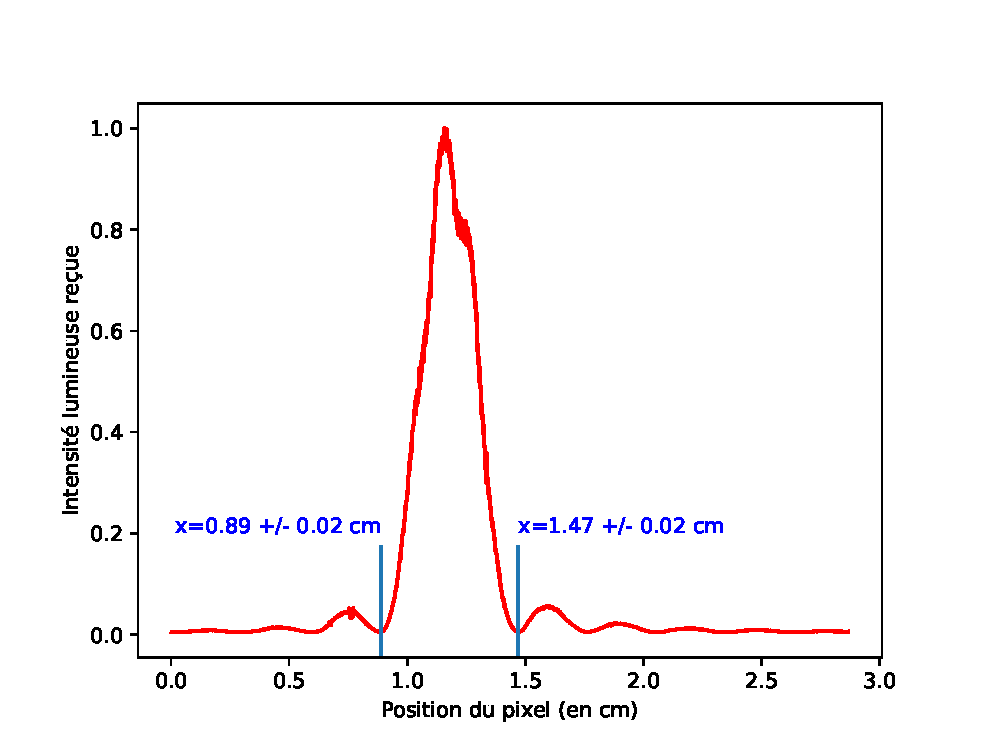
\includegraphics[scale=0.5]{img/graphe_camera_lineaire.eps}
    \end{center}
    \caption{Intensité en fonction de la position sur la cellule photo}
\end{figure}

Nous retrouvons le comportement approximatif du sinus cardinal, et nous pouvons obtenir avec une plus grande précision les deux points centraux des franges noires de chaque côté de la tâche centrale.
On obtient $x_1 = 0.89 \pm 0.02 cm$ et $x_2 = 1.47\pm 0.02 cm$, d'où $L_{exp} = \left\lvert x_2 - x_1 \right\rvert = 0.58 \pm 0.04 cm$. A partir de cette mesure, nous pouvons obtenir la taille de la fente connue, et l'on trouve
$a_{exp} = 150 \pm 11 \mu m$ (incertitude déterminée par la méthode de la dérivée). On retrouve la largeur de fente $a$ qu'on a utilisé.

\break
\subsection{Etude de différents motifs de diffraction}
Dans cette partie, nous souhaitons mettre en évidence des différences de comportement des figures de diffraction selon la forme de l'ouverture. 
Nous reprenons alors le montage de la figure (\ref{fig:montage_simple}), mais nous remplaçons la fente par un des motifs diffractifs présents sur le jeton A3000. 

\begin{figure}[h!]
    \centering
    \begin{subfigure}{.33\textwidth}
      \centering
        \includegraphics[width=.7\linewidth]{img/motifs/IMG_9174 (Personnalisé).png}
      \caption{Ouverture plus petite}
    \end{subfigure}%
    \begin{subfigure}{.33\textwidth}
      \centering
      \includegraphics[width=.7\linewidth]{img/motifs/IMG_9175 (Personnalisé).png}
      \caption{Ouverture initiale}
    \end{subfigure}
    \begin{subfigure}{.33\textwidth}
        \centering
        \includegraphics[width=.7\linewidth]{img/motifs/IMG_9176 (Personnalisé).png}
        \caption{Ouverture plus grande}
    \end{subfigure}
    \caption{Figure de diffraction pour un trou simple}
    \label{fig:fig_trou_simple}
\end{figure}

Nous remarquons que plus le trou a un diamètre élevé, plus la tache centrale est petite, et on observe de plus en plus d'anneaux sur la figure de diffraction. La figure de diffraction
se présente non plus comme un enchainement de frange en ligne, mais sous forme d'anneaux.

Concernant le motif diffractif en carré, nous observons une figure de diffraction composée de carré, avec une taille de la tâche centrale de plus en plus petite lorsque la taille du carré diffractif augmente.

\begin{figure}[h!]
    \centering
    \begin{subfigure}{.5\textwidth}
      \centering
        \includegraphics[width=.4\linewidth]{img/motifs/IMG_9177 (Personnalisé).png}
      \caption{Ouverture plus petite}
    \end{subfigure}%
    \begin{subfigure}{.5\textwidth}
      \centering
      \includegraphics[width=.4\linewidth]{img/motifs/IMG_9178 (Personnalisé).png}
      \caption{Ouverture plus grande}
    \end{subfigure}
    \caption{Figure de diffraction par un carré}
    \label{fig:fig_carre}
\end{figure}

Enfin, on s'intéresse au cas d'un rectangle comme motif diffractif. On positionne l'écran à une distance $D = 79 \pm 0.8cm$ du jeton diffractif. Nous observons que la figure de diffraction forme un rectangle
de longueur $l = 1.3 \pm 0.1cm$ et de largeur $l' = 0.4 \pm 0.05cm$. Nous pouvons en déduire les dimensions du rectangle sur le motif diffractif d'après la formule (\ref{eqn:loi_L}), et on trouve que le motif diffractif doit avoir 
comme dimension $65 \pm 5 \mu m$ en largeur, et $210 \pm 27 \mu m$ en longueur, et sa taille théorique est de $70\times200 \mu m$. Les dimensions théoriques sont incluses dans les bornes de nos mesures avec les incertitudes.  
\break
\subsection{Théorème de Babinet et taille d'un cheveu}
Le théorème de Babinet donne que la figure de diffraction d'un objet et de son complémentaire est la même.
Ainsi, un fil et une fente de même épaisseur $a$ forment dont une seule et même figure d'interférence ayant la même largeur de tâche centrale. Cette propriété permet la mesure de longueur très petite, que nous allons utiliser
pour déterminer le diamètre d'un cheveu.

Pour illustrer le théorème, nous positionnons le jeu de fente A3015 à une distance $D = 77.4 \pm 0.5 cm$ d'un écran. 
On éclaire une fente d'une largeur $a$ avec un laser de longueur d'onde $\lambda = 532 \pm 10nm$. On mesure la largeur de la tâche centrale, puis l'on éclaire le fil de même épaisseur $a$ en dessous de la fente précédente.
Nous remarquons que les largeurs $L$ des tâches centrales entre la fente et le fil sont identiques à l'incertitude près.

On commence par positionner un laser de longueur d'onde $\lambda = 532 \pm 10 nm$ face à un écran. A l'aide d'un support de diapositive (ayant un cheveu scotché dessus) que l'on place à une distance $D = 77.4 \pm 0.5 cm$ de
l'écran, on mesure la largeur de la tâche centrale $L$. 

\begin{figure}[!h]
    \begin{center}
        \resizebox{0.6\textwidth}{8cm}{
        \begin{tikzpicture}[x=0.75pt,y=0.75pt,yscale=-1,xscale=1]
    %uncomment if require: \path (0,429); %set diagram left start at 0, and has height of 429

    %Flowchart: Process [id:dp7587016517098488] 
    \draw   (110,120) -- (190,120) -- (190,140) -- (110,140) -- cycle ;
    %Straight Lines [id:da1423603054270386] 
    \draw [color={rgb, 255:red, 208; green, 2; blue, 27 }  ,draw opacity=1 ][line width=0.75]    (190,130) -- (360,130) ;
    \draw [shift={(281,130)}, rotate = 180] [color={rgb, 255:red, 208; green, 2; blue, 27 }  ,draw opacity=1 ][line width=0.75]    (10.93,-3.29) .. controls (6.95,-1.4) and (3.31,-0.3) .. (0,0) .. controls (3.31,0.3) and (6.95,1.4) .. (10.93,3.29)   ;
    %Straight Lines [id:da16631230033992783] 
    \draw    (360,140) -- (360,180) ;
    %Straight Lines [id:da6025420297783186] 
    \draw    (360,80) -- (360,120) ;
    %Straight Lines [id:da364809732100976] 
    \draw [color={rgb, 255:red, 208; green, 2; blue, 27 }  ,draw opacity=1 ]   (360,130) -- (540,110) ;
    \draw [shift={(455.96,119.34)}, rotate = 173.66] [color={rgb, 255:red, 208; green, 2; blue, 27 }  ,draw opacity=1 ][line width=0.75]    (10.93,-3.29) .. controls (6.95,-1.4) and (3.31,-0.3) .. (0,0) .. controls (3.31,0.3) and (6.95,1.4) .. (10.93,3.29)   ;
    %Straight Lines [id:da29487712829226687] 
    \draw [color={rgb, 255:red, 208; green, 2; blue, 27 }  ,draw opacity=1 ]   (360,130) -- (540,150) ;
    \draw [shift={(455.96,140.66)}, rotate = 186.34] [color={rgb, 255:red, 208; green, 2; blue, 27 }  ,draw opacity=1 ][line width=0.75]    (10.93,-3.29) .. controls (6.95,-1.4) and (3.31,-0.3) .. (0,0) .. controls (3.31,0.3) and (6.95,1.4) .. (10.93,3.29)   ;
    %Straight Lines [id:da5859877642355407] 
    \draw  [dash pattern={on 0.84pt off 2.51pt}]  (360,130) -- (540,130) ;
    %Straight Lines [id:da8840842764785435] 
    \draw    (540,80) -- (540,180) ;
    %Straight Lines [id:da5130608383839474] 
    \draw    (372,220) -- (528,220) ;
    \draw [shift={(530,220)}, rotate = 180] [color={rgb, 255:red, 0; green, 0; blue, 0 }  ][line width=0.75]    (10.93,-3.29) .. controls (6.95,-1.4) and (3.31,-0.3) .. (0,0) .. controls (3.31,0.3) and (6.95,1.4) .. (10.93,3.29)   ;
    \draw [shift={(370,220)}, rotate = 0] [color={rgb, 255:red, 0; green, 0; blue, 0 }  ][line width=0.75]    (10.93,-3.29) .. controls (6.95,-1.4) and (3.31,-0.3) .. (0,0) .. controls (3.31,0.3) and (6.95,1.4) .. (10.93,3.29)   ;
    %Straight Lines [id:da9345083369474423] 
    \draw    (560,112) -- (560,148) ;
    \draw [shift={(560,150)}, rotate = 270] [color={rgb, 255:red, 0; green, 0; blue, 0 }  ][line width=0.75]    (10.93,-3.29) .. controls (6.95,-1.4) and (3.31,-0.3) .. (0,0) .. controls (3.31,0.3) and (6.95,1.4) .. (10.93,3.29)   ;
    \draw [shift={(560,110)}, rotate = 90] [color={rgb, 255:red, 0; green, 0; blue, 0 }  ][line width=0.75]    (10.93,-3.29) .. controls (6.95,-1.4) and (3.31,-0.3) .. (0,0) .. controls (3.31,0.3) and (6.95,1.4) .. (10.93,3.29)   ;
    %Flowchart: Process [id:dp0037548894552708045] 
    \draw   (110,280) -- (190,280) -- (190,300) -- (110,300) -- cycle ;
    %Straight Lines [id:da6846741364957676] 
    \draw [color={rgb, 255:red, 208; green, 2; blue, 27 }  ,draw opacity=1 ][line width=0.75]    (190,290) -- (360,290) ;
    \draw [shift={(281,290)}, rotate = 180] [color={rgb, 255:red, 208; green, 2; blue, 27 }  ,draw opacity=1 ][line width=0.75]    (10.93,-3.29) .. controls (6.95,-1.4) and (3.31,-0.3) .. (0,0) .. controls (3.31,0.3) and (6.95,1.4) .. (10.93,3.29)   ;
    %Straight Lines [id:da021706815786682876] 
    \draw [color={rgb, 255:red, 208; green, 2; blue, 27 }  ,draw opacity=1 ]   (360,290) -- (540,270) ;
    \draw [shift={(455.96,279.34)}, rotate = 173.66] [color={rgb, 255:red, 208; green, 2; blue, 27 }  ,draw opacity=1 ][line width=0.75]    (10.93,-3.29) .. controls (6.95,-1.4) and (3.31,-0.3) .. (0,0) .. controls (3.31,0.3) and (6.95,1.4) .. (10.93,3.29)   ;
    %Straight Lines [id:da044428076418244755] 
    \draw [color={rgb, 255:red, 208; green, 2; blue, 27 }  ,draw opacity=1 ]   (360,290) -- (540,310) ;
    \draw [shift={(455.96,300.66)}, rotate = 186.34] [color={rgb, 255:red, 208; green, 2; blue, 27 }  ,draw opacity=1 ][line width=0.75]    (10.93,-3.29) .. controls (6.95,-1.4) and (3.31,-0.3) .. (0,0) .. controls (3.31,0.3) and (6.95,1.4) .. (10.93,3.29)   ;
    %Straight Lines [id:da4536520815231391] 
    \draw  [dash pattern={on 0.84pt off 2.51pt}]  (360,290) -- (540,290) ;
    %Straight Lines [id:da2719763791486136] 
    \draw    (540,240) -- (540,340) ;
    %Straight Lines [id:da9223524271493639] 
    \draw    (560,272) -- (560,308) ;
    \draw [shift={(560,310)}, rotate = 270] [color={rgb, 255:red, 0; green, 0; blue, 0 }  ][line width=0.75]    (10.93,-3.29) .. controls (6.95,-1.4) and (3.31,-0.3) .. (0,0) .. controls (3.31,0.3) and (6.95,1.4) .. (10.93,3.29)   ;
    \draw [shift={(560,270)}, rotate = 90] [color={rgb, 255:red, 0; green, 0; blue, 0 }  ][line width=0.75]    (10.93,-3.29) .. controls (6.95,-1.4) and (3.31,-0.3) .. (0,0) .. controls (3.31,0.3) and (6.95,1.4) .. (10.93,3.29)   ;
    %Shape: Circle [id:dp9133941073673402] 
    \draw  [fill={rgb, 255:red, 0; green, 0; blue, 0 }  ,fill opacity=1 ] (355,290) .. controls (355,287.24) and (357.24,285) .. (360,285) .. controls (362.76,285) and (365,287.24) .. (365,290) .. controls (365,292.76) and (362.76,295) .. (360,295) .. controls (357.24,295) and (355,292.76) .. (355,290) -- cycle ;
    %Straight Lines [id:da8477820676507002] 
    \draw    (360,340) -- (360,302) ;
    \draw [shift={(360,300)}, rotate = 90] [color={rgb, 255:red, 0; green, 0; blue, 0 }  ][line width=0.75]    (10.93,-3.29) .. controls (6.95,-1.4) and (3.31,-0.3) .. (0,0) .. controls (3.31,0.3) and (6.95,1.4) .. (10.93,3.29)   ;

    % Text Node
    \draw (131,122) node [anchor=north west][inner sep=0.75pt]   [align=left] {Laser};
    % Text Node
    \draw (311,29) node [anchor=north west][inner sep=0.75pt]   [align=left] {Fente simple\\de largeur $\displaystyle a$};
    % Text Node
    \draw (518,361) node [anchor=north west][inner sep=0.75pt]   [align=left] {Ecran};
    % Text Node
    \draw (444,192.4) node [anchor=north west][inner sep=0.75pt]    {$D$};
    % Text Node
    \draw (571,122.4) node [anchor=north west][inner sep=0.75pt]    {$L_{a}$};
    % Text Node
    \draw (131,282) node [anchor=north west][inner sep=0.75pt]   [align=left] {Laser};
    % Text Node
    \draw (292,349) node [anchor=north west][inner sep=0.75pt]   [align=left] {Cheveu de diamètre\\$\displaystyle d_{cheveu}$ à déterminer};
    % Text Node
    \draw (571,282.4) node [anchor=north west][inner sep=0.75pt]    {$L_{cheveu}$};
    % Text Node
    \draw (521,42) node [anchor=north west][inner sep=0.75pt]   [align=left] {Ecran};
\end{tikzpicture}
        }
    \end{center}
    \caption{Schéma du protocole}
\end{figure}

On obtient une tâche centrale $L_1 = 1.5 \pm 0.05cm$ pour un cheveu du premier expérimentateur, et $L_2 = 0.75 \pm 0.05cm$ pour le second expérimentateur, on peut donc remonter à l'épaisseur du cheveu en utilisant la formule:
\begin{align}
    d_{cheveu} = \frac{2 \lambda D}{L}
\end{align}

Nous obtenons alors $d_{cheveu,1} = 55 \pm 2 \mu m$ et $d_{cheveu,2} = 110 \pm 8 \mu m$. Le premier cheveu étant connu fin, et le second épais, les mesures sont en accord. De plus, les valeurs restent dans les intervalles
fournies par la littérature, bien que étant chacune dans les extremums.
\section{Diffraction par des ouvertures multiples}
Dans cette partie nous étudierons les figures de diffractions pour des ouvertures doubles puis des ouvertures multiples. Nous étudierons ensuite les figures de diffractions d'objets du quotidien pour les caractériser. 

\subsection{Diffraction par des ouvertures doubles}
\subsection{Modèle}
L'intensité totale résultante de deux fentes est donnée par:

\begin{equation}
I(\theta)=I_0 sinc^2 \left(\frac{\pi a \sin(\theta)}{\lambda}\right) \cos^2 \left(\frac{\pi d \sin(\theta)}{\lambda}\right)
\label{equa:Intensité_doubles}
\end{equation}
$I_0$ est l'intensité maximale, $\lambda$ est la longueur d'onde de la source, $a$ est la largeur des fentes,$d$ est le distance entre les fentes et $\theta$ est l'angle d'observation.
La longueur de la tâche centrale reste la même que pour une fente simple $L=\frac{2 \lambda D}{a}$ avec D la distance entre les fentes et l'écran. L'interfrange i est donnée par :

\begin{equation}
    i= \frac{\lambda D}{d}
\label{equa:interfrange}
\end{equation}

\subsection{Protocole expérimental}
On fait passer notre laser par un jeton diffractif ayant des fentes doubles (fentes d'Young) ou des trous doubles (trous d'Young). UTILISATION LENTILLE? La longueur d'onde du laser est $\lambda = 532 \pm 10 nm$. On observe les figures d'interférences d'abord sur un écran puis on utilise une caméra linéaire pour mesurer $i$ et $L$. On suppose que la caméra est précise au pixel près ???, notre incertitude sur $L$ et $i$ est donc égale à la largeur d'un pixel qui vaut $14 \mu m$. On mesure la distance $D$ entre les fentes grâce à une règle. Le jeton étant large et comme nous ne savons pas où sont placées les fentes sur le jeton, on estime l'incertitude $\delta D= 0.8 cm$. 

\subsection{Observations et interprétations}


\subsubsection{Fentes d'Young}

\subsubsection{Trous d'Young}

\subsection{Diffraction par un réseau}


\subsection{Modèle}
L'intensité totale est donnée par:
\begin{equation}
    I(\theta)=\frac{I_0}{N^2}sinc^2(\frac{\pi a sin \theta}{\lambda})(\frac{sin(N\frac{\pi d sin \theta}{\lambda})}{sin(\frac{\pi d sin \theta}{\lambda})})^2
\end{equation}

$d$ est la distance entre 2 fentes, qu'on appelle pas du réseau. Les formules pour $L$ et $i$ restent les mêmes pour des fentes multiples. 

\subsection{Protocole expérimental}
On utilise le même protocole que pour des fentes doubles mais on change de jeton diffractif. On commence par faire varier  le nombre de fentes, puis on fait varier le pas du réseau. Ensuite on fait varier la longueur d'onde du laser.

\subsection{Observations et interprétations}

\subsubsection{Étude de l'influence du nombre de fente éclairées}

\subsubsection{Étude de l'influence du pas du réseau sur la figure de diffraction}

\subsubsection{Étude de l'influence de la longueur d'onde sur la figure de diffraction d'un réseau}

\subsection{Caractérisation d'un objet du quotidien}
\newpage

\section*{Annexes}
\subsection{Démonstration sans approximation des petits angles}
Nous avons $\sin \theta = \frac{y}{\sqrt{D^2+y^2}}$ ce qui nous donne alors:
\begin{align*}
    \sin \theta = \frac{n\lambda}{a} & \Leftrightarrow \frac{y}{\sqrt{D^2+y^2}} = \frac{n\lambda}{a} \\
    & \Leftrightarrow a^2y^2 = n^2 \lambda ^2 \left( D^2 + y^2 \right) \\
    & \Leftrightarrow y^2 = \frac{n^2 \lambda^2 D^2}{a^2 - n^2 \lambda^2} \\
    & \Leftrightarrow y = \pm \frac{n \lambda D}{\sqrt{a^2 - n^2 \lambda^2}}
\end{align*}

Enfin, dans l'approximation où $\lambda \ll a$, nous avons :
\begin{align}
    y = \pm \frac{n \lambda D}{a}
\end{align}

On retrouve bien l'approximation des petits angles.

\end{document}
